% \documentclass[margin=0mm]{standalone}
% \input{../tikz_header}


% \begin{document}





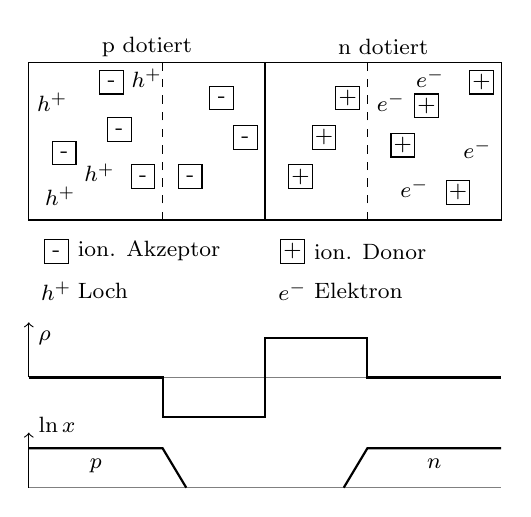
\begin{tikzpicture}[font=\footnotesize]
  %\useasboundingbox (0,0) rectangle (5,5);
  %\draw (11,10) rectangle ++(5,5);
  
  \node at (1.5, 2.2) {p dotiert};
  \node at (4.5, 2.2) {n dotiert};

  \draw (0,0) rectangle ++ (3,2);
  \draw (3,0) rectangle ++ (3,2);
  \draw[dashed] (1.7,0) -- ++ (0,2);
  \draw[dashed] (4.3,0) -- ++ (0,2);
  

  %-------------
  \draw (1,1) rectangle node {-} ++ (0.3, 0.3);
  \draw (0.3,0.7) rectangle node {-} ++ (0.3, 0.3);
  \draw (1.3,0.4) rectangle node {-} ++ (0.3, 0.3);
  \draw (0.9,1.6) rectangle node {-} ++ (0.3, 0.3);

  \node at (0.3,1.5) {$h^+$};
  \node at (0.4,0.3) {$h^+$};
  \node at (1.5,1.8) {$h^+$};
  \node at (0.9,0.6) {$h^+$};

  %--------------
  
  \draw (1.9,0.4) rectangle node {-} ++ (0.3, 0.3);
  \draw (2.3, 1.4) rectangle node {-} ++ (0.3, 0.3);
  \draw (2.6,0.9) rectangle node {-} ++ (0.3, 0.3);


    %--------------
  
    \draw (3.9,1.4) rectangle node {+} ++ (0.3, 0.3);
    \draw (3.3, 0.4) rectangle node {+} ++ (0.3, 0.3);
    \draw (3.6,0.9) rectangle node {+} ++ (0.3, 0.3);
  
  %--------------
  
  \draw (5.6,1.6) rectangle node {+} ++ (0.3, 0.3);
  \draw (5.3, 0.2) rectangle node {+} ++ (0.3, 0.3);
  \draw (4.6,0.8) rectangle node {+} ++ (0.3, 0.3);
  \draw (4.9,1.3) rectangle node {+} ++ (0.3, 0.3);

  \node at (4.6,1.5) {$e^-$};
  \node at (4.9,0.4) {$e^-$};
  \node at (5.1,1.8) {$e^-$};
  \node at (5.7,0.9) {$e^-$};

%---------

\draw (0.2,-0.55) rectangle node {-} ++ (0.3, 0.3);
\node[right] at (0.5, -0.4) {ion. Akzeptor};

\node at (0.35,-0.9) {$h^+$};
\node[right] at (0.5, -0.9) {Loch};



\draw (3.2,-0.55) rectangle node {+} ++ (0.3, 0.3);
\node[right] at (3.5, -0.4) {ion. Donor};

\node at (3.35,-0.9) {$e^-$};
\node[right] at (3.5, -0.9) {Elektron};


%-------------------

\begin{scope}[yshift = -20mm]
  \draw[gray] (0,0) -- (6,0);
  \draw[->] (0,0) -- (0,0.7) node[right, yshift=-2mm] {$\rho$};

  \draw[thick] (0,0) -- (1.7,0) -- (1.7,-0.5) -- (3,-0.5) -- (3, 0.5) -- (4.3, 0.5) -- (4.3, 0) -- (6,0);

\end{scope}

%-------------------

\begin{scope}[yshift = -34mm]
  \draw[gray] (0,0) -- (6,0);
  \draw[->] (0,0) -- (0,0.7) node[right, yshift=1mm] {$\ln x$};

  \draw[thick] (0,0.5) -- node[below] {$p$} ++ (1.7,0) -- ++ (0.3, - 0.5);
  \draw[thick] (6,0.5) -- node[below] {$n$} ++ (-1.7,0) -- ++ (-0.3, - 0.5);

\end{scope}


\end{tikzpicture}

%\end{document}